\documentclass[11pt,a4paper]{article}
\usepackage[T1]{fontenc}
\usepackage{lmodern}
\usepackage[margin=2.5cm]{geometry}
\usepackage{amsmath}
\usepackage{graphicx}
\usepackage{booktabs}
\usepackage{siunitx}
\usepackage{pgfplots}
\pgfplotsset{compat=1.16}
\usepackage[hidelinks]{hyperref}
\usepackage{cleveref}

\title{Experiment 3: Free Fall and the Acceleration of Gravity}
\author{Your Name \\ Lab partner: Partner Name}
\date{Performed: \today \quad Course: PHYS 101}

\begin{document}
\maketitle

\begin{abstract}
Two or three sentences: what you measured, the value you found with its uncertainty,
and whether it agrees with the accepted value.
\end{abstract}

\section{Aim}
State the question the experiment answers. Here: determine $g$ from the fall time of a
steel ball over several heights.

\section{Theory}
Write down the equations you use and define every symbol. For free fall from rest,
\begin{equation}
  h = \tfrac{1}{2} g t^{2}, \qquad\text{so}\qquad t^{2} = \frac{2}{g}\, h .
  \label{eq:fall}
\end{equation}
A straight line of $t^2$ against $h$ therefore has the slope $2/g$.

\section{Method}
List the apparatus and what you did, in the past tense and in enough detail for someone
else to repeat it: a steel ball ($m = \SI{28}{g}$), a release magnet, a photogate timer
(resolution \SI{0.1}{ms}) and a metre rule (resolution \SI{1}{mm}). The height was varied
from \SI{0.20}{m} to \SI{1.00}{m}; each height was timed five times.

\section{Results}
\Cref{tab:data} gives the mean times and \cref{fig:fit} the fit of \cref{eq:fall}.
\texttt{siunitx} keeps numbers and units consistent, and aligns table columns on the decimal point.

\begin{table}[ht]
  \centering
  \caption{Mean fall time for each height (five runs each).}
  \label{tab:data}
  \begin{tabular}{S[table-format=1.2] S[table-format=1.4] S[table-format=1.4]}
    \toprule
    {$h$ (\si{m})} & {$\bar t$ (\si{s})} & {$\sigma_t$ (\si{s})} \\
    \midrule
    0.20 & 0.2021 & 0.0004 \\
    0.40 & 0.2858 & 0.0005 \\
    0.60 & 0.3498 & 0.0006 \\
    0.80 & 0.4041 & 0.0006 \\
    1.00 & 0.4519 & 0.0007 \\
    \bottomrule
  \end{tabular}
\end{table}

\begin{figure}[ht]
  \centering
  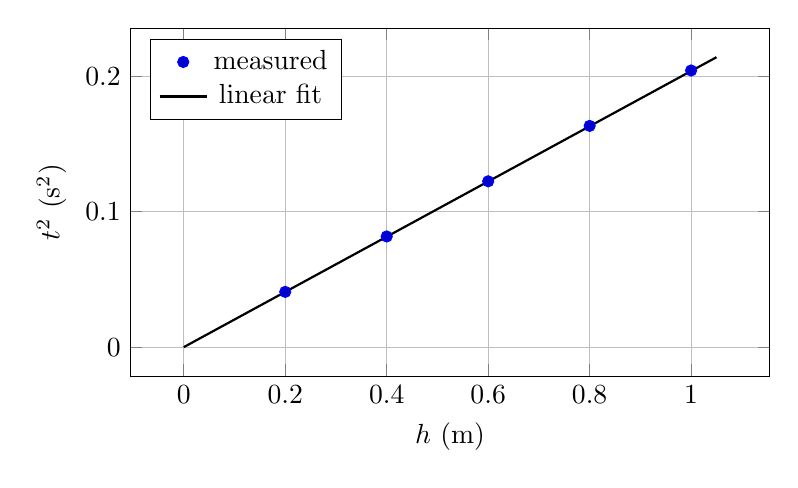
\begin{tikzpicture}
    \begin{axis}[width=0.8\linewidth, height=6cm, xlabel={$h$ (m)}, ylabel={$t^2$ (s$^2$)},
                 grid=major, legend pos=north west]
      \addplot+[only marks] coordinates {(0.2,0.0408) (0.4,0.0817) (0.6,0.1224) (0.8,0.1633) (1.0,0.2042)};
      \addplot[domain=0:1.05, thick] {0.2038*x};
      \legend{measured, linear fit}
    \end{axis}
  \end{tikzpicture}
  \caption{$t^2$ against $h$. The slope of the fit is \SI{0.2038}{s^2/m}.}
  \label{fig:fit}
\end{figure}

From the slope, $g = 2/\text{slope} = \SI{9.81 \pm 0.05}{m/s^2}$.

\section{Discussion}
Compare with the accepted value ($\SI{9.81}{m/s^2}$) and say whether they agree within
the uncertainty. List the main sources of error (release delay, air drag, ruler reading)
and how each would change the result. Suggest one improvement.

\section{Conclusion}
One sentence with the result and its uncertainty.

\end{document}
